\section{The \texorpdfstring{$G=5$}{G=5} and \texorpdfstring{$G=11$}{G=11} towers}\label{sec:towers}
The class theorems of \cref{sec:regimes} determine an orbit once the first-event times of its stages are known. Two infinite families of fresh stages can be solved completely; they are the objects whose topology is studied in \cref{sec:towertop}. In both, ``one tower step'' replaces $S_k$ by $S_{k+1}$ and corresponds to one period of the orbit.

\subsection{The \texorpdfstring{$G=11$}{G=11} tower}
\begin{theorem}[$\ell=11$: period $8$, multiplier $9$]\label{thm:R3T5bp}
For $k\ge0$ let $S_k=2^2\,3^{3+k}\,5^4$ and $x=S_k^2/11$. Then $G(x)=11$, $L(x)=S_k$, $|D(x)|=2k+7$, and the orbit satisfies
\[
x_{8k+j}=\frac{(j+1)\,S_k^2}{11}\quad(0\le j\le8),\qquad x_{n+8}=9\,x_n,\qquad G(x_n)=11\ \text{for all }n,
\]
with exactly one occurrence event per period (at $j=8$), which creates exactly two new elements of $D$.
\end{theorem}
\prov{CW-0418}{R3-T5b'}{PROVED}{FULL}
\begin{proof}
\emph{Occurrence set.} Modulo $11$ the element $2$ is a primitive root and $3=2^8$, $5=2^4$. For $d=2^a3^c5^e$ with $a\le2$, $c\le3+k$, $e\le4$ we get $d\equiv2^{a+8c+4e}$, so $d\equiv1$ iff $a+8c+4e\equiv0\pmod{10}$. This forces $a$ even, $a\in\{0,2\}$; for $a=0$ it reads $e\equiv-2c\pmod5$, for $a=2$ it reads $e\equiv2-2c\pmod5$. For each of the $2(k+4)$ pairs $(a,c)$ there is exactly one $e\in[0,4]$. Removing $d=1$ leaves $|D|=2k+7$ (and $d\le S_k$ always has $d^2\mid S_k^2$). Since $12=2^2\cdot3\in D$ and every $d-1$ is divisible by $11$, $G=11$. The maximal exponents occur: $2^2$ in $12$; $5^4$ with $a=0,c=3$ ($e\equiv-6\equiv4$); and $3^{3+k}$ with $a=0$ and $e\equiv-2(3+k)$. Hence $L=S_k$.

\emph{One period.} By \cref{thm:R3T5a} the states while $D$ is unchanged are $x_t=tS_k^2/11$ ($t=j+1$), valid as long as $11\nmid t+1$, which holds for $t\le8$. By the proof of \cref{thm:R3T5b}, $D(x_t)=D_{11}(u_tS_k)$ with $u_t\in\{1,2\}$ for $t\le8$. The factor $2$ only raises the exponent of $2$ to $3$, which is odd and never a solution, so $D_{11}(2S_k)=D_{11}(S_k)$ and $D$ is constant for $t\le8$. At $t=9$, $u_t=3$ and the exponent of $3$ becomes $4+k$; the new solutions have $c=4+k$, one $e$ for each $a\in\{0,2\}$: exactly two new elements, and $L'=3S_k=S_{k+1}$. So $x_8=9S_k^2/11=S_{k+1}^2/11$, and the claim follows by induction on $k$ (the fresh-stage hypothesis holds at every $k$). \qedhere
\end{proof}
\Cref{fig:g11cycle} shows one period of the $G=11$ tower.
\begin{figure}[tbp]\centering
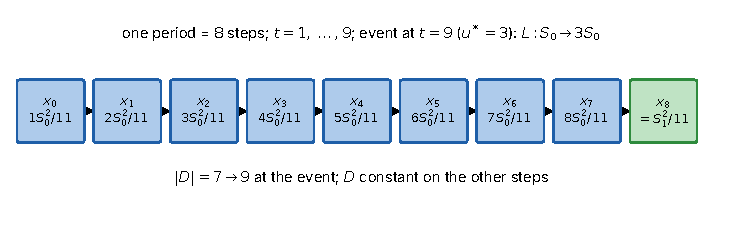
\includegraphics[width=\textwidth]{fig09_g11_cycle}
\caption{\textbf{One period of the $G=11$ tower (exact; proved by \cref{thm:R3T5bp}).} Parameters: $S_0=2^2\,3^3\,5^4$, $\ell=11$. The nine states $x_0..x_8$ of one period are drawn as boxes; $t=1,\dots,9$, the only event is at $t=9$ ($u^*=3$) where $L$ passes from $S_0$ to $3S_0$ and $|D|$ from $7$ to $9$. The orbit is abstract (arithmetic); the geometric consequence is studied in \cref{sec:towertop}.}\label{fig:g11cycle}
\end{figure}

\subsection{The \texorpdfstring{$G=5$}{G=5} tower and the failure of the converse}
\begin{theorem}[$\ell=5$: period $3$, multiplier $4$]\label{thm:R3T5c}
For $k\ge0$ let $S_k=126\cdot2^k=2^{k+1}\,3^2\,7$ and $x=S_k^2/5$. Then $G(x)=5$, $L(x)=S_k$ and
\[
x_{3k+j}=\frac{(j+1)\,S_k^2}{5}\quad(0\le j\le3),\qquad x_{n+3}=4\,x_n,\qquad G(x_n)=5\ \text{for all }n,
\]
with one event per period, at $t=4$, which creates $1$ or $2$ new elements of $D$ according as $-(k+2)\bmod4\in\{1,2\}$ or $\{0,3\}$.
\end{theorem}
\prov{CW-0419}{R3-T5c}{PROVED}{FULL}
\begin{proof}
Modulo $5$, $2$ is a primitive root, $3=2^3$ and $7\equiv2$, so $d=2^a3^c7^f\equiv2^{a+3c+f}$, which is $1$ iff $a+3c+f\equiv0\pmod4$. We have $6\in D$ ($a=1,c=1$), so $G=5$. The maximal exponents occur: for $7^1$ take $(a,c)=(0,1)$; for $3^2$ take $(a,f)=(1,1)$ ($1+6+1=8$); for $2^{k+1}$ one needs $3c+f\equiv-(k+1)\pmod4$ with $c\in\{0,1,2\}$, $f\in\{0,1\}$, and $3c+f$ takes the residues $0,1,3,0,2,3$, i.e.\ all residues. Hence $L=S_k$. The values $t=2,3$ are squarefree so $u_t=1$ and $D$ is unchanged, and $5\nmid t+1$ for $t\le3$. At $t=4$, $u_t=2$ and the exponent of $2$ rises to $k+2$; the new elements have $a=k+2$ and $3c+f\equiv-(k+2)$, which has $2,1,1,2$ solutions for the residues $0,1,2,3$ respectively. So $L'=2S_k=S_{k+1}$ and $x_3=4S_k^2/5=S_{k+1}^2/5$. \qedhere
\end{proof}
\begin{corollary}[B2-T7 is not an equivalence]\label{cor:B2T7}
The orbit of $126^2/5$ is rigid in the sense of \cref{def:rigid} with $G_\infty=5$.
\end{corollary}
\Cref{fig:g5cycle} shows one period of the $G=5$ tower.
\begin{figure}[tbp]\centering
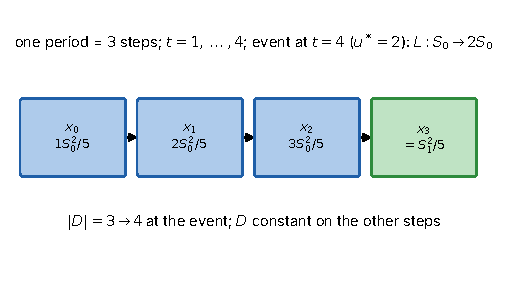
\includegraphics[width=\textwidth]{fig08_g5_cycle}
\caption{\textbf{One period of the $G=5$ tower (exact; proved by \cref{thm:R3T5c}).} Parameters: $S_0=126$, $\ell=5$. Boxes: $x_0..x_3$ with $t=1,\dots,4$; the event at $t=4$ ($u^*=2$) takes $L$ from $S_0$ to $2S_0$ and $|D|$ from $3$ to $4$. Same period and multiplier as the integer rigid orbit, but with $G=5$ rather than $1$ (\cref{fig:rigid}).}\label{fig:g5cycle}
\end{figure}

\subsection{Stage law and the \texorpdfstring{$\ell=29$}{l=29} control}
\begin{theorem}[stage law; periodic stage sequences]\label{thm:R3T5d}
Suppose an orbit in the class $G=\ell$ is a concatenation of fresh stages with first-event times $\tau_i=u_i^2$ and $L_{i+1}=u_iL_i$. Then stage $i$ lasts $\tau_i-1$ steps and multiplies $x$ by $\tau_i$. If the sequence $(\tau_i)$ is periodic with period $r$, then
\[
x_{n+P}=\rho^2x_n\ \ (n\ge n_0),\qquad P=\sum_{i<r}(\tau_i-1),\quad\rho^2=\prod_{i<r}\tau_i .
\]
The towers above are the cases $(\tau)=(9)$: $(P,\rho^2)=(8,9)$, and $(\tau)=(4)$: $(3,4)$.
\end{theorem}
\prov{CW-0420}{R3-T5d}{MIXED}{SPLIT}
\begin{proof}
At the start of stage $i$ the state is $L_i^2/\ell$; at its end, by \cref{thm:R3T5b}, it is $\tau_iL_i^2/\ell=L_{i+1}^2/\ell$. Inside a stage the state at offset $s$ is $(1+s)L_i^2/\ell$. If $\tau_{i+r}=\tau_i$ for all $i$ then $L_{i+r}=\rho L_i$ and the states of stage $i+r$ are those of stage $i$ multiplied by $\rho^2$, with the same stage lengths. \qedhere
\end{proof}
\begin{example}[$\ell=29$, $S=1890$; finite-exact]\label{ex:l29}
For $x_0=1890^2/29$ the first-event times are $\tau=(25,4,9)$ over three stages, so $P=24+3+8=35$ and $\rho^2=900$. Events occur at steps $24,27,35,59,62,70$; $x_{35}=900\,x_0$, $x_{70}=900\,x_{35}$; $G\equiv29$ throughout; the first event creates the single element $175$. This was checked with the independent engine for two full periods; \emph{periodicity for all further stages is verified, not proved}, which is why the record is split (stage law proved given periodicity; the instance finite-exact).
\end{example}
\begin{remark}[cited census]
A census of $1{,}920$ orbits $x_0=S^2/\ell$, $\ell\in\{5,\dots,29\}$ prime, of $70$--$90$ steps found among the persistent ($G>1$ forever) periodic orbits only the pairs $(P,\rho^2)=(3,4),(8,9),(35,900)$. This is \stat{cited} from the source release, not re-run, and is not a theorem.
\end{remark}
